\chapter{Ciele práce}

V učiacich sa systémoch založených na predkladnaní dvojíc vstup - požadovaný výstup
je možné stanoviť chybu a tú vhodnými metódami minimalizovať.
V prípade systému s odmeňovaním sa požaduje od výstupu výkonnej jednotky postupnosť
akcií, ktoré maximalizujú celkovú odmenu.
Príkladom môže byť rozhodovanie robota, ktorý má splniť cieľ pozostávajúci z
niekoľkých elementárnych úkonov, ale postupnosť týchto elementárnych úkonov nie je známa -
nie je teda definovaná požadovaná hodnota výstupu.
Riešením tohto problému je zavedenie systému odmeňovania agenta (robota) \ref{img:reinforcement_learning}.

\begin{figure}[!htb]
\center
\includegraphics[scale=.8]{../diagrams/agent.png}
\caption{Učenie s odmeňovaním}
\label{img:reinforcement_learning}
\end{figure}

Odmena je získaná z prostredia po vykonaní akcie. Ohodnotenie akcie v danom stave
je tvorené predošlými skúsenosťami z vykonania predošlých akcií a získania odmien.
Podstatou učenia je teda ohodnotenie vykonaných akcií v danom stave aby bolo
možné v každom stave rozhodnúť, ktorá akcia je najlepšia - vyberá sa teda
postupnosť akcií $\pi$ pre ktorú je funkcia

\begin{equation}
\Lambda(\pi)  = \sum\limits_{n=0}^{L(\pi)}\gamma^n P_{\pi(n)}(s(n), s(n-1))
\label{eq:q_quality}
\end{equation}

Agent ako jednotka schopná konať rozhodnutia (akcie) v prostredí danom Markovovim \cite{bib:markov_02}
rozhodovacím procesom hľadá optimálnu stratégiu v zmysle rovnice \ref{eq:q_quality}.
maximálna. Kde $\gamma \in \langle 0, 1 \rangle$ je koeficient zabúdania, $P_{\pi(n)}{(s(n), s(n-1)}$
je odmeňovacia funkcia po prechode zo stavu $s(n-1)$ do stavu $s(n)$ vykonaním $\pi(n)$ a
$L(\pi)$ je dĺžka postupnosti $\pi$


Cieľom agenta je teda nájsť optimálnu stratégiu a maximalizovať tak odmenu.
Pre veľký počet stavov je hľadanie optima metódou počítania
pravdepodobností prechodov medzi stavmi $P(s, s')$ ťažko vypočítateľné.

Východiskom sú napríklad algoritmy Q-learning, alebo SARSA. Tieto algoritmy počítajú
ohodnotenie akcie v danom stave $Q(s(n), a(n))$, ktoré číselne vyjadruje vhodnosť
danej akcie. Využitie môžu nájsť \cite{bib:q_app_01}, \cite{bib:q_app_02}, \cite{bib:q_app_03} napríklad pri plánovnaí rozhodnutí v
\begin{enumerate}
  \item robotike
  \item virtuálnych agentových systémoch
  \item počítačové hry
\end{enumerate}

Vo všobecnosti riešia uvedené algoritmy problémy umelej inteligencie, kedy
nie je možné zostaviť trénovacie dáta v tvare vstup, požadovaný výstup a aplikácia
je obmedzená na udeľovanie odmien agentovi za vykonanie zvolenej stratégie
\cite{bib:reinforcement_leraning_01}, \cite{bib:reinforcement_leraning_02}. Na rozdiel
od evolučných algoritmov (genetické algoritmy, diferenciálna evolúcia, simulované žíhanie),
kedy je daná kriteriálna funkcia, umožňujú algoritmy Q-learning, alebo SARSA
postupne zlepšovať riešenie na princípe hľadania optimálnej stratégie z niekoľkých
optimálnych podstratégií - už nájdené optimálne riešenie podstratégie sa nemení. V prípade evolučných
algoritmov je typická zmena všetkých hľadaných parametrov. Nie sú teda vhodné
na úlohy kde sa požaduje generovanie postupnosti akcií.

Pre algoritmus Q-learning je zaručená konvergencia k optimálnemu
ohodnoteniu (v zmysle \ref{eq:q_quality}) \cite{bib:q_conv_proof}
pre ľubovolnú metódu výberu
akcií - postačuje aby každá akcia mala nenulovú pravdpodobnosť vykonania v prislúchajúcom
stave. V prípade SARSA táto konvergencia nie je zaručená pre všetky metódy výberu akcií.
Oba algoritmy pracujú v diskrétnom čase.

Pre problémy s rádovo stovkami stavov, ktoré sú diskrétne, môže byť fukcia $Q(s(n), a(n))$ realizovaná
formou tabuľky. Konvergencia k optimálnemu riešeniu je v tomto prípade zaručená.
Pre problémy kde je počet stavov veľmi veľký (tisíce a viac), alebo stavy nenadobúdajú
diskrétne hodnoty je potrebné zvoliť aproximáciu tejto funkcie. Konvergencia v tomto
prípade už nie je zaručená.

Prístupov ako aproximovať túto funkciu je niekoľko \cite{bib:aproximation_01},
\cite{bib:aproximation_02}, \cite{bib:aproximation_03}, \cite{bib:aproximation_04}.
Najčastejšie používané
\begin{enumerate}
  \item Diskretizácia stavov spojitých hodnôt tabuľkou
  \item Lineárna kombinácia príznakov
  \item Dopredná neurónová sieť
  \item Neurónová sieť bázických funkcií
\end{enumerate}

Prvý spôsob predstavuje triviálne riešnie problému redukciou nekonečného
počtu stavov na konečný.

Druhý spôsob spočíva v pevne definovaných príznakoch, ktoré závisia od typu
problému. Tieto príznaky tvoria súbor funkcií $f_{i}(s(n),a(n))$. Hodnota $Q(s(n), a(n))$
je daná lineárnou kombináciou týchto príznakov. Hľadá sa teda vektor váh
$w$ pre ktorý  $Q_b(s(n), a(n), w) = \sum\limits_{i=0}^{I}w_i f_{i}(s(n),a(n))$
má minimálnu veľkosť chyby $e$, definovaná je ako
$e(w) = \sum\limits_{s,a} (Q(s(n), a(n))- Q_b(s(n), a(n), w))^2$
Problematická zostáva voľba príznakových funkcií - ich tvar aj počet.

Tretí spôsob spočíva v použití doprednej neurónovej siete ako univerzálny aproximátor funkcie.
Schopnosť aproximovať funkciu doprednou neurónovou sieťou je veľmi dobre známa aj preskúmaná.
Pre úlohy Q-learning algoritmu je však nepoužiteľná \cite{bib:q_fnn_problem},
z dôvodov nemožnosti túto sieť naučiť doteraz dostupnými prostriedkami. Hoci existuje niekoľko prípadov kde sa učenie dá
uskutočniť, vo všeobecnosti sú v protiklade dva požiadavky :
\begin{enumerate}
  \item Učenie siete na požadovanú hodnotu
  \item Generovanie požadovanej hodnoty
\end{enumerate}

Sieť teda musí zároveň poskytovať správny výstup pre minulé stavy a zároveň sa
učiť na súčastný stav bez toho, aby sa hodnoty z minulých stavov zmenili.

Štvrtý spôsob je využíva lineárnu kombináciu bázických funkcie.
Bázické funkcie sú dané vopred, avšak ich parametre sa menia v priebehu učenia,
podobne ako vektor váh lineárnej kombinácie $w$. Nech sú ich parametre označené
ako $v$. Cieľom je nájsť také $w$ a $v$ pre ktoré chyba
$e(v, w) = \sum\limits_{s,a}(Q(s(n), a(n))- Q_b(s(n), a(n), v, w))^2$
je minimálna. Kde $Q_b(s(n), a(n), v, w) = \sum\limits_{i=0}^{I}w_i f_{i}(s(n),a(n), v_i)$.

{\bf Cieľom práce} je overiť možnosti aproximácie funkcie $Q(s(n), a(n))$
uvedenými metódami. Vzľadom na už prebehnutý výskum a problémy dopredných
neurónových sieti, sa problematika sústredí najmä
na hľadanie vhodných bázických funkcií. Práve v tejto oblasti je venovaný výskumu
najväčší priestor. Tieto funkcie by mali byť volené tak, aby zmena parametrov $v_i$ jednej
funkcie, neovplivnila výsledok inde ako pre žiadané $s(n)$ a $a(n)$.
Použité riešnie je potom možné využiť vo veľkých stavových priestorov, kde možnosti použiť tabuľku
zlyhávajú z dôvodov
\begin{enumerate}
  \item Veľké pamäťové nároky
  \item Nutnosť navštíviť a správne spočítať Q pre všetky $s(n)$, $a(n)$
\end{enumerate}
Prvý problém nepredstavuje pre súčasné počítače až tak veľký nedostatok tabuľkového
riešenia. Horšia je situácia v prípade vypĺňania korektných hodnôt v tabuľke. Práve rekurentnou
povahou algoritmov Q-learning a SARSA je časovo veľmi náročné vyplniť tieto hodnoty -
mnohonásobne treba navštíviť všetky stavy a vykonať v nich všetky akcie. Práve to je
primárny dôvod aproximovať funkciu $Q(s(n), a(n))$.


\section{Q-learning algoritmus}

Q-learning algoritmus je definovaný pre časovo diskrétne systémy.
Agent ktorý prechádza stavový priestor vykonaním niektorej z vopred daných
akcií získava za tieto prechody odmeny. Cieľom algoritmu je ohodnotiť všetky akcie
v jednotlivých stavoch, tak aby bol dosiahnutý ustálený stav a v každom stave
bolo možno vybrať akciu prinášajúcu najväčšiu odmenu, v zmysle
s \ref{eq:q_quality}.

\subsection{Definícia algoritmu}

Autorom Q-learning algoritmu je Christopher J.C.H. Watkins, v roku 1992 publikoval
článok kde tento algoritmus predstavil \cite{bib:q_learning_watkins} a niekoľko ďalších
vysvetlení tohto algoritmu je možné nájsť v \cite{bib:q_tutorial_01} alebo
\cite{bib:q_tutorial_02}. Dôkazy o konvergencií k otimálnemu riešeniu (v zmysle
s \ref{eq:q_quality}) sú k dispozícií \cite{bib:q_proof_01}, \cite{bib:q_proof_02},
\cite{bib:q_proof_03}, \cite{bib:q_proof_04}.
\\
Je daná odmeňovacia funkcia $R(s(n),a(n))$, ktorá vyjadruje okamžité ohodnotenie konania
agenta v stave $s(n)$ vykonaním akcie $a(n)$. V reálnych aplikáciach táto funkcia nadobúda takmer v každom
$s(n)$ a $a(n)$ hodnotu $0$. Pre správnu funkciu algoritmu, musí byť aspoň jedna hodnota
nenulová - napr. ohodnotenie dosiahnutia cieľového stavu (samotná existencia cieľového
stavu však pre algoritmus nie je potrebná).

Funkcia ohodnotení je definovaná ako

\begin{equation}
Q_{n}(s(n),a(n)) = R(s(n),a(n)) + \gamma \max_{a(n-1) \in \mathbb{A}} Q_{n-1}(s(n-1), a(n-1))
\label{eq:q_learning}
\end{equation}

\begin{itemize}
 \item $R(s(n),a(n))$ je odmeňovacia funkcia
 \item $Q_{n-1}(s(n-1),a(n-1))$ je funkcia ohodnotení v stave $s(n-1)$ pre akciu $a(n-1)$
 \item $\gamma$ je odmeňovacia konštanta a platí $\gamma \in (0, 1)$.
\end{itemize}

Funkcia $\ref{eq:q_learning}$ definuje ohodnotenie akcií vo všetkých stavoch t.j.
agent, ktorý sa dostal do stavu $s(n)$ vykonaním akcie $a(n)$ zo stavu
$s(n-1)$ získal odmenu $R(s(n),a(n))$ a zlomok najväčšieho možného ohodnotenia, ktoré
mohol získať dostaním sa do stavu $s(n-1)$, situáciu ilustruje obrázok \ref{img:q_learning}.

\begin{figure}[!htb]
\center
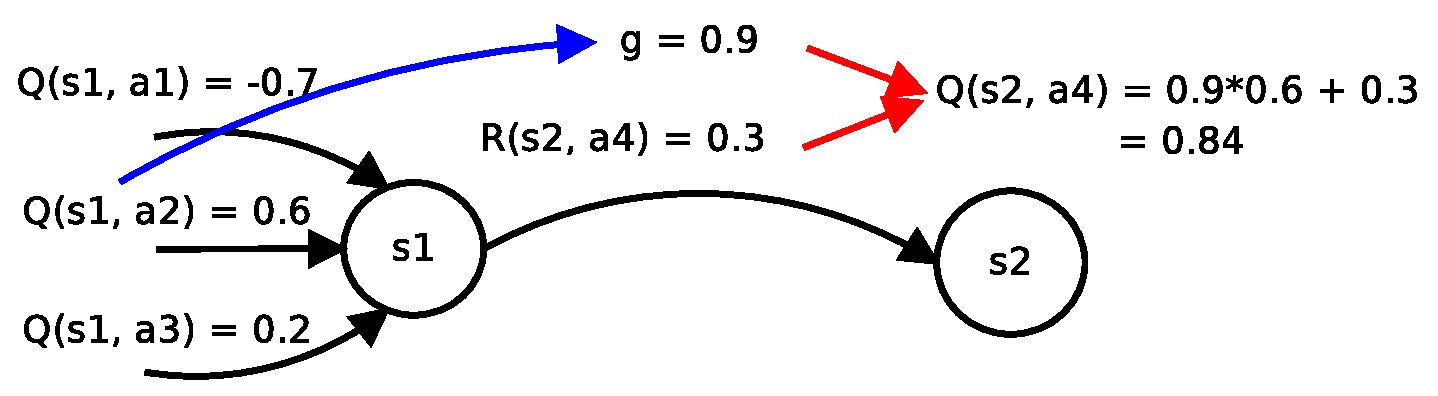
\includegraphics[scale=.6]{../diagrams/q_learning_detail.eps}
\caption{Ilustrácia funkcie ohodnotení, pre $\gamma = 0.9$}
\label{img:q_learning}
\end{figure}

Je potrebné poznamenať, že práve časť $\max_{a(n-1) \in \mathbb{A}} Q_{n-1}(s(n-1), a(n-1)$
zabezpečuje nezávislosť konvergencie k optimu bez ohľadu voľby stratégie výberu akcie -
postačuje, aby každá akcia, v každom stave mala nenulovú pravdepodobnosť vykonania.
Určitým variantom je algoritmus SARSA \cite{bib:sarsa}

\begin{align}
Q_{n}(s(n),a(n)) &= \nonumber \\
 (1-&\alpha)Q_{n-1}(s(n),a(n)) + \nonumber  \\
&\alpha(R(s(n),a(n)) + \gamma Q_{n-1}(s(n-1), a(n-1)))
\label{eq:sarsa}
\end{align}

kde $\alpha \in (0, 1)$, hodnota $Q_{n}(s(n),a(n))$ sa  teda ustáli na strednej hodnote
a závisí od stratégie výberu akcií. Q-learning teda vychádza z toho, čo najlepšie sa mohlo stať
a SARSA z toho čo sa naozaj stalo.


\chapter{Navrhnuté bázické funkcie neurónovej siete pre aproximáciu}

Vhodnú funkciu je možné zmenou parametrov upraviť do tvaru, aby pre zvolený
vstup $I_0(n)$ dosahovala požadovanú hodnotu a postupným zväčšovaním
vzdialenosti $\mid I_0(n) - I_i(n) \mid$ klesala jej hodnota k nule.

Najjednoduhším príkladom takýchto funkcií  je

\begin{equation}
f_j(X(n)) =
\left\{
	\begin{array}{ll}
		k_j  & ak \ X(n) = X^j_0 \\
		0 & inak
	\end{array}
\right.
\label{eq:bfnn_simple}
\end{equation}

kde $k_j$ je hodnota požadovaná v bode $X^j_0$. Výstupom siete potom je

\begin{align}
y(X) = \sum\limits_{j=1} f_j(X(n))
\label{eq:bfnn_simple_res}
\end{align}

Z charakteru Q-learning algoritmu majú hodnoty $Q(s(n),a(n))$ charakter
postupne klesajúcich hodnôt. Je teda potrebné vybrať iné funkcie.

Nasledujú preto definície funkcií s ktorými boli urobené experimenty.

Dané sú bázické funkcie $f_j^x(\boldmath{s(n), a(n)})$, kde $x$ je typ bázickej funkcie.
Požadovaná hodnota $Q^x(s(n), a(n))$ je potom lineárnou kombináciou týchto funkcií typu $x$.

Z charakteru Q-learning algoritmu \ref{eq:q_learning} je možné určiť požiadavky na
tieto funkcie :

\begin{enumerate}
\item predpis \ref{eq:q_learning} je tvorený klesajúcou exponenciálou - podobný charakter by mala mať aj bázická funkcia
\item existencia jedného globálneho maxima a zmenou parametrov určovať polohu tohto bodu
\item možnosť ľubovolne meniť strmosť funkcie v okolí maxima
\item funkcia by mala byť zhora aj z dola ohraničená
\end{enumerate}

Cieľom je mať možnosť nezávisle nastaviť maximá funkcií do oblastí, ktoré zodpovedajú
nenulovím hodnotám $R(s(n), a(n))$ - bod 2. Ak ohodnotenie spĺňa podmienku najlepšej
možnej akcie v danom stave, dá sa očakávať že bude mať menšiu strmosť, naopak, ak funkcia
popisuje bod kde $R(s(n), a(n))$ dosahuje malé hodnoty (obvykle záporné), bude požadovaná
vysoká strmosť tejto funkcie - obe požiadavky sú zhrnuté v bode 3. Bod 4 umožňuje rozumne
ohraničiť rozsah funkcie.

Niektoré tvary bázických funkcií ktoré možno uvažovať pre problém aproximácie
\begin{align}
    f_j^1(\boldmath{s(n), a(n)}) &= e^{ -\sum\limits_{i=1}^{n_s}{\beta_{aji}(n)(s_i(n) - \alpha_{aji}(n))^2} }  \\
    f_j^2(\boldmath{s(n), a(n)}) &= \frac{1}{1 + \sum\limits_{i=1}^{n_s}{\beta_{aji}(n)(s_i(n) - \alpha_{aji}(n))^2}}  \\
    f_j^3(\boldmath{s(n), a(n)}) &= e^{ -\sum\limits_{i=1}^{n_s}{\beta_{aji}(n)\mid s_i(n) - \alpha_{aji}(n) \mid} }
    \label{eq:basis_functions_01}
\end{align}

kde \\
$\alpha_{aji}(n) \in \langle -1, 1 \rangle$ určuje polohu maxima funkcie \\
$\beta_{aji}(n) \in (0, \infty)$ určuje strmosť funkcie.

Ich priebehy pre prvé dve uvedené sú na obrázku \ref{img:basis_funcions}.

\begin{figure}[]
\center
\includegraphics[scale=.4]{../pictures/gaussian_1D.png}
\caption{Znázornenie priebehov bázických fukcií}
\label{img:basis_funcions}
\end{figure}

Pre symetrické prechody medzi stavmi ich možno zjednodušiť na

\begin{align}
f_j^1(\boldmath{s(n), a(n)}) &= e^{ -\beta_{aj} \sum\limits_{i=1}^{n_s}{(s_i(n) - \alpha_{aji})^2} }  \\
f_j^2(\boldmath{s(n), a(n)}) &= \frac{1}{1 + {\beta_{aj} \sum\limits_{i=1}^{n_s}(s_i(n) - \alpha_{aji})^2}}  \\
f_j^3(\boldmath{(n)s, a(n)}) &= e^{ -\beta_{aj} \sum\limits_{i=1}^{n_s}{\mid s_i(n) - \alpha_{aji}(n) \mid} }
\label{eq:basis_functions}
\end{align}

Aproximovaná funkcia ohodnotení pre $l$ bázických funkcií je potom

\begin{align}
Q^x(s(n), a(n)) = \sum\limits_{j=1}^{l} w(n)_j^x f_j^x(\boldmath{s(n), a(n)})
\label{eq:knn_y_update}
\end{align}

kde $w(n)_j^x$ sú váhy bázických funkcií.


Je teda potrebné stanoviť celkovo 3 sady parametrov : $\alpha$ $\beta$ $w$.

\subsection{Určenie parametrov $\alpha$}

Parameter $\alpha$ určuje posunutie maxima funkcie a postupuje sa podobne
ako v prípade \ref{eq:knn_w_update}. Treba zohľadniť fakt, že pre konečný
výsledok je dôležité pokryť všetky oblasti s nenulovým $R(s(n),a(n))$, vrchol
krivky bude ležať nad nad bodom $[s(n),a(n)]$.

Zmena parametrov $\alpha$ prebieha v piatich krokoch.

\begin{itemize}
  \item na začiatku sa zvolia $\alpha_{jia}(n)$ náhodne, ze $\langle -1, 1 \rangle$
  \item spočítajú sa vzdialenosti od predloženého vstupu $d_{ja}(n) = \mid s(n) - \alpha_{ja}(n) \mid$
  \item nájde sa také $ka$ kde pre $\forall{j} : d_{ka}(n) \leq d_{ja}(n)$
  \item spočíta sa krok učenia $\eta'_a(n) = \eta_1 \mid Q_r(s(n), a(n)) \mid$
  \item upravia sa parametre $\alpha_{aki}(n+1) = (1 - \eta')\alpha_{aki}(n) + \eta' s_{i}(n)$
\end{itemize}
kde \\
$Q_r(s(n), a(n))$ je požadovaný výstup \\
$\eta_1$ je konštanta učenia

Krok učenia teda závisí od veľkosti požadovanej hodnoty, tým sa zabezpečí aby maximum
krivky naozaj ležalo nad bodom $[s(n),a(n)]$.

\subsection{Určenie parametrov $\beta$}

Parameter $\beta$ určuje strmosť krivky. Ak boli k dizpozicií naraz všetky
požadované výstupy, bolo by možné spočítat tento parameter z rozptylu.
Požadované hodnoty však prichádzajú postupne, strmosť krivky sa preto upravuje priebežne,
podľa toho či požadovaná hodnota leží nad, alebo pod krivkou.

\begin{itemize}
\item stanoví sa chyba $e(n) = Q_r(s(n), a(n)) - Q(s(n), a(n))$
\item pre každú bázickú funkciu  $\beta_{ja}(n+1)= \beta_{ja}(n) + \eta_2 e(n)w_{ja}(n)$
\item skontroluje sa $\beta_{ja}(n) \in (0, \infty)$
\end{itemize}

kde \\
$Q_r(s(n), a(n))$ je požadovaný výstup \\
$\eta_2$ je konštanta učenia \\


\subsection{Určenie váhových parametrov $w$}

Nakoniec sa gradientovou metódou určia váhové paramete. Pre presné
riešenie by bolo možné použiť metódu nejmenších štvorcov, tá je však pre veľký počet
bázcikých funkcií ťažko vypočítateľná. Zmena parametrov je potom daná nasledujúcim postupom

\begin{itemize}
\item stanoví sa chyba $e(n) = Q_r(s(n), a(n)) - Q(s(n), a(n))$
\item pre každé $w_{ja}$ : $w_{ja}(n+1)= w_{ja}(n) + \eta_3 e(n)y_j(n)$
\item skontroluje sa $w_{ja}(n) \in (-r, r)$
\end{itemize}

kde \\
$\eta_3$ je konštanta učenia \\
$r$ je maximálny rozsah váh \\

\subsection{Hybridný variant}

Ak by funkcia $R(s(n), a(n))$ mala len jednu kladnú hodnotu a ostatné by boli
nulové, aproximáciu $Q(s(n), a(n))$ by veľmi dobre popísala Gaussova krivka \ref{eq:basis_functions}.
Ak by funkcia $R(s(n), a(n))$ mala len záporné hodnoty a ostatné by boli
nulové, funkcia $Q(s(n), a(n))$ by s ohliadnutím na \ref{eq:q_learning}
si boli rovné. Vo funkcí $Q(s(n), a(n))$ by sa tak objavilo niekoľko záporných
hodnôt, ostro ohraničených.

Vyjduc z týchto úvah, je možné skombinovať výhody oboch : Gaussova krivka
ktorá dokáže pokryť nenulovými hodnotami celý definyčný obor a má
možnosť tak šíriť hodnoty Q na ďalšie stavy a funkcie \ref{eq:bfnn_simple}.
Funkcia \ref{eq:bfnn_simple} predstavuje vlastne tabuľku, ktorá nadobúda
nenulové hodnoty vo vybraných bodoch - tvorí tak adaptívnu tabuľku.

Je teda možné skombinovať funkciu \ref{eq:bfnn_simple} s niektorou z \ref{eq:basis_functions},
čo vedie na vzťahy

\begin{align}
P_i(s(n), a(n)) &=
\left\{
	\begin{array}{ll}
		r_{ai}  & if \ s(n) = \alpha^1_i \\
		0 & inak
	\end{array}
\right. \\
  H_j(s(n), a(n)) &= w_{aj} e^{ -\beta_{aj} \sum\limits_{i=1}^{n_s}{(s_i(n) - \alpha^2_{aji})^2 }} \\
  Q(s(n), a(n)) &= \sum\limits_{i=1}^{I} P_i(s(n),a(n)) + \sum\limits_{j=1}^{J} H_j(s(n), a(n))
  \label{eq:peak_hill}
\end{align}

kde \\
$\alpha^1_j$ sú oblasti kde $H_j(s(n))$ nadobúda nenulové hodnoty \\
$\alpha^2_j$ sú oblasti pre ktoré $f_j(\boldmath{s(n), a(n)})$ nadobúda maximum \\
$r_{ai}$ je hodnota zápornej odmeny $R(s(n), a(n))$ \\
$w_{aj}$ je váha a zobovedá veľkosti maxima resp. minima pre fukciu \\
$\beta_{aj}$ je strmosť, a platí $\beta > 0$ \\
$I$ a $J$ sú počty bázických funkcií \\

Označenia $P$ a $H$ vznikli z tvaru funkcií : peak a hill. Funkcia bude na ďalších
grafoch označená ako Gauss + AT : kombinácia Gaussovej krivky a adaptívnej tabuľky.
Mechanizmus učenia zostáva rovnaký ako pre bázické funkcie v predošlej časti. Ukážka
priebehu funkcie pre dve premenné je na obrázku \ref{img:peak_hill_funcion}.
Počet funkcií $P_i(s(n), a(n))$ bol zvolený 30 a počet funkcií $P_i(s(n), a(n))$ 20.
Pre názornosť boli parametre $r_{ai}$ zvolené záporné a parametre $\beta_{aj}$ kladné.

Funkcia \label{eq:peak_hill} predstavuje nový tvar bázických funkcií pre
aproximovanie funkcie ohodnotení $Q(s(n), a(n))$.

\begin{figure}[]
\center
\includegraphics[scale=.5]{../pictures/peak_hill_function.png}
\caption{Znázornenie predmetnej funkcie}
\label{img:peak_hill_funcion}
\end{figure}
